\documentclass{article}
% Left align stuff
\usepackage[utf8]{inputenc}
\usepackage[english]{babel}
\usepackage[document]{ragged2e}
% other stuff
\usepackage{graphicx}
\usepackage[margin=1in]{geometry}
\PassOptionsToPackage{hyphens}{url}\usepackage{hyperref}
\usepackage{graphicx}
\usepackage{float}
\restylefloat{table}

\begin{document}

\title{Command and Control Subsystems Report}
\author{Jake Vossen: OREPACKAGERS}

\maketitle

% \begin{abstract}
% The abstract text goes here.
% \end{abstract}

\section{Subsystem Description}
The Command and Control subsystem is the subsystem responsible for
converting the requests that have been collected into downloaded data
to be distributed to users. It starts by receiving a list of
\texttt{request} objects - a structure for contating information about
each request. To prevent confusion, the mono-spaced \texttt{request}
will refer to they Python object itself, wheras plain ``request''
refers to the concept of a user request.

With this list of requests, the first thing it does is use Pythons
\texttt{multiprocessing}[1] library to split work up between the
different threads on the computer. While this software is designed
for low end machines to be more accessable to developing areas, most
computers[2] in recent times will have more than 1 CPU core (including
the Raspberry Pi[3]). This allows for the processor to split up all
the requests, and execute them in paralel, instead of waiting for each
one to finish individually, which can provide a large preformance
boost.

When downloading a \texttt{request}, it determens the type of
request. The types are URL, search, youtube, and ipfs. It follows this
flow chart to decide what to do:

\begin{figure}[h]
  \centering
  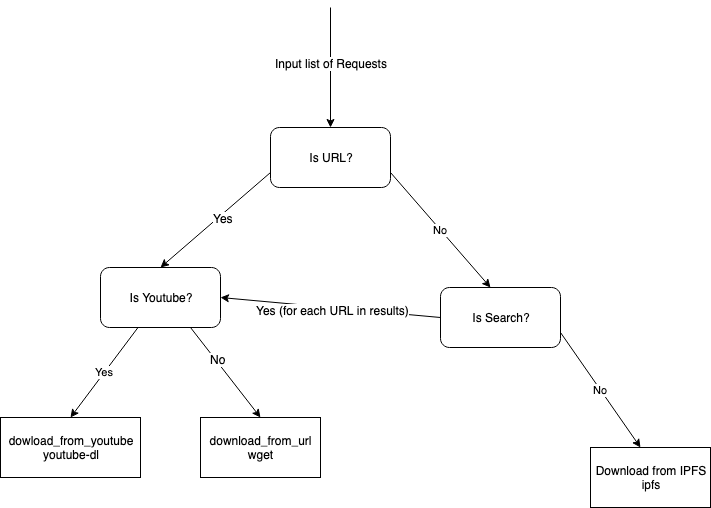
\includegraphics[scale=.6]{log-flow-chart.png}
  \caption{\begingroup \fontsize{10pt}{12pt}\selectfont Diagram describing flow chart of downloading each
    \texttt{request}. Jake Vossen, 2019-04-01 \endgroup}
\end{figure}

The steps for each type of request is outlined below.

\subsection{URLs}

URLs are your basic websites, such as
\url{https://en.wikipedia.org/wiki/Monty_Python_and_the_Holy_Grail},
or
\url{https://www.nytimes.com/2019/03/27/technology/turing-award-ai.html}. This
is for users who already know the content they want. In the backend,
the Python program is going to use the \texttt{wget}[4]
utility. Specifically, \texttt{wget -E -H -k -K -p -P path url
  robots=off} where \texttt{path} is the output directory and
\texttt{url} is the url that has been requested. To break it down:
\begin{itemize}
  \item \texttt{-E} tells \texttt{wget} to change the file extention
    if the url isn't a .html file. This allows for the downloading of
    PDF files as well as HTML files
  \item \texttt{-H} Tells \texttt{wget} that it is okay to download
    material from hosts that aren't from the specified URL. While this
    seems backwards at first, many websites host their fonts or
    pictures in a place that isn't the same as the document that is
    being request. This allows the page to appear just as it would
    when visited in a web browser
  \item \texttt{-k} This stands for ``convert links'', which means
    that when the download is complete, it converts the links on the
    page so they are sudible for browsing on the local machine. For
    example, if a blog has \texttt{otherwebsite.com/picture} on it, it
    will replace that with just \texttt{picture} to ensure that the
    browser will use the local versions of that picture
  \item \texttt{-K} This means that \texttt{wget} will make a backup
    of the HTML file when converting links with the \texttt{-k}
    option.
  \item \texttt{-p} is the most important option, as it tells
    \texttt{wget} to download all the requirements as well as the
    url. So if the site links to an outside source (such as
    \texttt{otherwebsite.com/picture}) also gets downloaded if it is
    linked in the requested url.
  \end{itemize}
All of those options ensures that downloading the URL requested get's
the website exactly as it appears in a browser, including linked
images. Additionally, it works with PDF and ZIP files, which is really
important to ensure all possible media can be obtained. This method is
also used by other parts of the program.

\subsection{Search}

Sometimes the user will not know exactly what they want, so we added
an option to get the first page of Google results (top 10
results). The \texttt{googlesearch}[5] library was very helpful for
this. This library provides a list of URLs, and then we use the URL
method to download those results (or the youtube download option if it
is a youtube link). The results are each in thier own folder nammed
based on the google search rank (1 is first result, 2 is second
result, etc). 

\subsection{YouTube}

It is well known that lot of quality educational and entiertainment
content is in video format, and the majority of that content is on
YouTube. That is why we are adding functionallity to request YouTube
videos (through a link, or a result from the search function). In this
case, the \texttt{youtube-dl} program allows for content retrevial.

\subsection{IPFS}
IPFS stands for ``InterPlanetary File System'', which is a ``A
peer-to-peer hypermedia protocol to make the web faster, safer, and
more open''[7]. The internet that is familiar to most people is the
client-server model[8], but IPFS changes that so everyone is both a
client and a server. Media is distribtued based of their crytographic
hash, a unique ID for each object instead of a URL. Anybody can add
objects, and when requesting an object, it can be downloaded from any
number of servers, not just the origional person hosting the
server. The \texttt{ipfs} command line utility[9] is used to retreive
objects.

\section{Interfaces with Other Subsystems}

Software is all about abstraction, so there are a handful of points in
which the Command and Control subsystem will interface with the other
subsystems. Ideally, all the other subsystems will work indepenedently
and a couple of links will get everything working together.

\subsection{Input - List of Requests}

Python only stores objects in memory while the program is
running. That means when the program is shut down (or the machine is
powered off), the data genereated must be saved somewhere on the
device or else that information would be lost. In this case, what is
important is to be able to store the \texttt{request} objects. This is
completed by the data managment subsystem. This means my subsystem
will call \texttt{get\_all\_requests()} which will retreive the data
about the requests, create the objects again (as they where destroyed
from memory when the program shut down), and return that information
to Command and Control.

\subsection{Output - Download path and status}

Once my subsystem completes it's donwload, it needs to update the
database about the new status. This is again through the Data
Managment subsystem. To ensure we only download each object once, each
\texttt{request} has two properties: \texttt{file\_location} and
\texttt{downloaded\_status}. Once Command and Control has completed a
download, it will call the Data Managment method
\texttt{update\_request(r)} where \texttt{r} include the changes to
\texttt{file\_location} and \texttt{downloaded\_status}. So the
Data Managmnet subsystem knows which database entry to update, we use
a Universily Uniquie Identifier (UUID)[10] to identify each
request.

\begin{figure}[h]
  \centering
  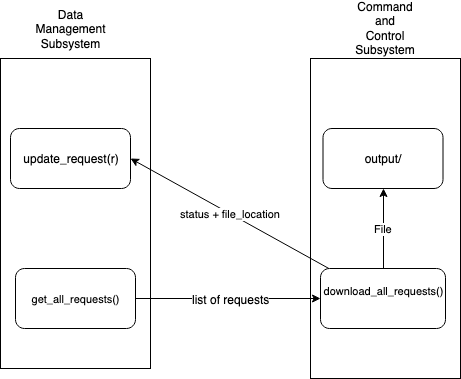
\includegraphics[scale=.5]{input-output.png}
  \caption{\begingroup \fontsize{10pt}{12pt}\selectfont Diagram
    describing the inputs and outputs of the Command and Control sub-system
    \texttt{request}. Jake Vossen, 2019-04-01 \endgroup}
\end{figure}

\section{Stakeholder Considerations}

\section{Validation}

Testing is one of the most fundamentally important things in software
development. It is easy to write code, but it is not useful if it
can't work under a variety of difficult tests. A handful of curated
tested designed to test the bounderies of the code have been
picked. To verify the results, there are two primary methods. The
first, is a SHA-512 sum, which is a crytographically secure way to
ensure two files are the same[11]. The first file origionatty from a
manual download, and the second one from the Command and Control
Subsystem. If the two hashes are the same, the subsystem was
successful. However, this cannot be used for all
tests, because when downloading from a webiste, the origional HTML files
are modified for browsing offline (see the \texttt{-k} option on
wget. This makes it impossible to cryptographically ensure that the
requested file is thhe same as the downloaded file, so a visual
analysis is preformed to analize the two documents and ensure that
they are identical. The table below explains the tests preformed,
where the ``Analysis Method'' is either visual or hash to preform the
check. 

% Please add the following required packages to your document preamble:
% \usepackage{graphicx}
\begin{table}[H]
\centering
\caption{\begingroup \fontsize{10pt}{12pt}\selectfont Tests Preformed
Jake Vossen, 2019-04-01 \endgroup}
\label{my-label}
\resizebox{\textwidth}{!}{%
\begin{tabular}{l|l|l|l|l}
Type   & Value                                                                                     & Expected Result                                       & Analysis Method & Expected = Actual? \\ \hline
URL    & https://www.gutenberg.org/cache/epub/2265/pg2265.txt                                      & Text of ``Hamlet" By Shakesphere                       & Hash            & Yes                \\ \hline
URL    & https://static.googleusercontent.com/media/research.google.com/en//pubs/archive/46507.pdf & PDF of Google Machine Learning Research Paper         & Hash            & Yes                \\ \hline
URL    & https://en.wikipedia.org/wiki/Monty\_Python\_and\_the\_Holy\_Grail                        & Wikipedia entry for ``Monty Python and the Holy Grail" & Visual          & Yes                \\ \hline
youtube & https://www.youtube.com/watch?v=dQw4w9WgXcQ
                                                                                                   & Rick Roll                                 & Visual          & Yes                \\ \hline
search & What Is the Airspeed Velocity of an Unladen Swallow?                                      & Google search results                                 & Visual          & Yes                \\ \hline
ipfs   & /ipfs/QmS4ustL54uo8FzR9455qaxZwuMiUhyvMcX9Ba8nUH4uVv/readme                               & IPFS introduction document                            & Hash            & Yes                \\ \hline
ipfs   & /ipfs/QmVLTMHtLRhnft3QspDx4qTJeXY6hiib1j77UfQmY54CGe/mosaic.png                           & 300 MB picture of the moon                            & Hash            & Yes               
\end{tabular}%
}
\end{table}

The other important validation is to ensure that the multithreading
described in section 1 improves results. I ran the program with 8
faily large requests and used the \texttt{time}[12] utility to measure
the runtime of the program. The results are shown below:

\begin{table}[H]
\centering
\caption{\begingroup \fontsize{10pt}{12pt}\selectfont Tests Preformed
Jake Vossen, 2019-04-01 \endgroup}
\label{my-label}
% \resizebox{\textwidth}{!}{%\begin{table}[]
\begin{tabular}{l|l|l|l}
                                      1 Core  & 2 Cores & 4 Cores & 8
                                                                    Cores
  \\ \hline
 161.277 & 53.927  & 45.984  & 46.448 
\end{tabular}
% }
\end{table}

\section{Appendix}
\begin{verbatim}
from request import Request
from user import user
from datetime import datetime
import subprocess
import os
from googlesearch import search
import youtube_dl
import multiprocessing
from multiprocessing import Pool

def download_all_requests(requests):
    threads_count = multiprocessing.cpu_count()
    # threads_count = 1
    # threads_count = 2    
    # threads_count = 4
    # threads_count = 8
    with Pool(threads_count) as p:
        p.map(download_request, requests)
    # The above code is the same as the code below, above will do it with as many threads as possible
    # for r in requests:
        # download_request(r)

def mkdir(path):
    if not os.path.exists(path):
        os.makedirs(path)    
def download_request(r):
    if r.kind == "URL": # we are dealing with a plain old HTTP request
        url = r.value
        path = "output/" + r.uuid
        download_from_url(url, path)
    if r.kind == "search":
        search_list = list(search(r.value, stop = 10))
        for i in range(len(search_list)):
            url = search_list[i]
            path = 'output/' + r.uuid + '/' + str(i + 1) + '/'
            if ('youtube' not in url): # Youtube vidoes are not going to be able to work, those will be for the youtube request
                download_from_url(url, path)
            else: #leaving this out for now
                download_from_youtube(url, path)
    if r.kind == "youtube":
        path = "output/" + r.uuid + '/'
        download_from_youtube(r.value, path)
    if r.kind == "ipfs":
        path = "output/" + r.uuid + '/'
        download_from_ipfs(r.value, path)

    # mark_as_downloaded(p) # this is where this function will intergrate with data

def download_from_url(url, path):
    mkdir(path)
    subprocess.call(r'wget -E -H -k -K -p ' '-P ' + path + ' ' +  url + ' robots=off', shell=True)
def download_from_youtube(url, path):
    mkdir(path)
    ydl_opts = {
        'outtmpl': path + '%(title)s'
    }
    with youtube_dl.YoutubeDL(ydl_opts) as ydl:
        ydl.download([url])
def download_from_ipfs(ipfs_hash, path):
    mkdir(path)
    subprocess.call(r'ipfs get ' + ipfs_hash + ' -o ' + path, shell=True)
def main():
    #get_all_requests()
    requests = []
    # tests
    requests.append(Request("URL", "https://www.gutenberg.org/cache/epub/2265/pg2265.txt", user("Jake", "Vossen", "jakevossen", "asdf"), datetime.now()))
    requests.append(Request("URL", "https://static.googleusercontent.com/media/research.google.com/en//pubs/archive/46507.pdf", user("Jake", "Vossen", "jakevossen", "asdf"), datetime.now()))
    requests.append(Request("URL", "https://en.wikipedia.org/wiki/Monty_Python_and_the_Holy_Grail", user("Jake", "Vossen", "jakevossen", "asdf"), datetime.now()))
    requests.append(Request("search", "What Is the Airspeed Velocity of an Unladen Swallow?", user("Jake", "Vossen", "jakevossen", "asdf"), datetime.now()))
    requests.append(Request("search", "Library of Congress", user("Jake", "Vossen", "jakevossen", "asdf"), datetime.now()))    
    requests.append(Request("youtube", "https://www.youtube.com/watch?v=NtrVwX1ncqk", user("Jake", "Vossen", "jakevossen", "asdf"), datetime.now()))
    requests.append(Request("youtube", "https://www.youtube.com/watch?v=Gbtulv0mnlU", user("Jake", "Vossen", "jakevossen", "asdf"), datetime.now()))
    requests.append(Request("ipfs", "/ipfs/QmS4ustL54uo8FzR9455qaxZwuMiUhyvMcX9Ba8nUH4uVv/readme", user("Jake", "Vossen", "jakevossen", "asdf"), datetime.now()))
    requests.append(Request("ipfs", "/ipfs/QmVLTMHtLRhnft3QspDx4qTJeXY6hiib1j77UfQmY54CGe/mosaic.png", user("Jake", "Vossen", "jakevossen", "asdf"), datetime.now()))    
    
    download_all_requests(requests)

main()
\end{verbatim}
\section{Bibliography}

[1] ``multiprocessing - Process-based parallelism,''
\textit{multiprocessing - Process-based parallelism - Python 3.7.3
  documentation}. [Online]. Available:
\url{https://docs.python.org/3.7/library/multiprocessing.html}. [Accessed:
03-Apr-2019].

[2] ``Hardware Survey - CPU Cores,'' \textit{Hardware Survey - CPU Cores}. [Online]. Available: \url{https://www.pcbenchmarks.net/number-of-cpu-cores.html}. [Accessed: 03-Apr-2019]. 

[3] ``Raspberry Pi 3 Model B,'' Raspberry Pi. [Online]. Available:
\url{https://www.raspberrypi.org/products/raspberry-pi-3-model-b/}. [Accessed:
03-Apr-2019].

[4] ``GNU Wget 1.20 Manual,'' \textit{GNU Wget 1.20
  Manual}. [Online]. Available:
\url{https://www.gnu.org/software/wget/manual/wget.html}. [Accessed:
03-Apr-2019].

[5] MarioVilas, ``MarioVilas/googlesearch,'' GitHub,
06-Mar-2019. [Online]. Available:
\url{https://github.com/MarioVilas/googlesearch}. [Accessed:
03-Apr-2019].

[6] Ytdl-Org, ``ytdl-org/youtube-dl'' GitHub,
03-Apr-2019. [Online]. Available:
\url{https://github.com/ytdl-org/youtube-dl/}. [Accessed:
03-Apr-2019].

[7] ``IPFS is the Distributed Web'' IPFS. [Online]. Available:
\url{https://ipfs.io/}. [Accessed: 03-Apr-2019].

[8] ``Client-Server Mode,'' [Online]. Available:
\url{https://web.cs.wpi.edu/~cs513/s07/week1-unixsock.pdf}. [Accessed:
02-Apr-2019].

[9] ``IPFS Documentation,'' \textit{Install IPFS – IPFS Documentation}. [Online]. Available: \url{https://docs.ipfs.io/introduction/install/}. [Accessed: 03-Apr-2019]. 

[10] ``A Universally Unique IDentifier (UUID) URN Namespace,''
\textit{IETF Tools}. [Online]. Available:
\url{https://tools.ietf.org/html/rfc4122.html}. [Accessed:
03-Apr-2019].

[11] C. H. Romie, ``Secure Hash Standard (SHS)'' Aug-2015. [Online]. Available: \url{https://nvlpubs.nist.gov/nistpubs/FIPS/NIST.FIPS.180-4.pdf}. [Accessed: 02-Apr-2019].

[12] ``time,'' \textit{time(1) - OpenBSD manual pages}. [Online]. Available: https://man.openbsd.org/time. [Accessed: 03-Apr-2019].


\end{document}

%[1] https://docs.python.org/3.7/library/multiprocessing.html
%[2] https://www.pcbenchmarks.net/number-of-cpu-cores.html
%[3] https://www.raspberrypi.org/products/raspberry-pi-3-model-b/
%[4] https://www.gnu.org/software/wget/manual/wget.html
%[5] https://github.com/MarioVilas/googlesearch
%[6] https://github.com/ytdl-org/youtube-dl/
%[7] https://ipfs.io/
%[8] https://web.cs.wpi.edu/~cs513/s07/week1-unixsock.pdf
%[9] https://docs.ipfs.io/introduction/install/
%[10] https://tools.ietf.org/html/rfc4122.html
%[11] https://nvlpubs.nist.gov/nistpubs/FIPS/NIST.FIPS.180-4.pdf
%[12] https://developer.apple.com/download/more/
%[13] https://man.openbsd.org/time